\section*{Question 4}
\begin{wrapfigure}{r}{0.35\textwidth}
    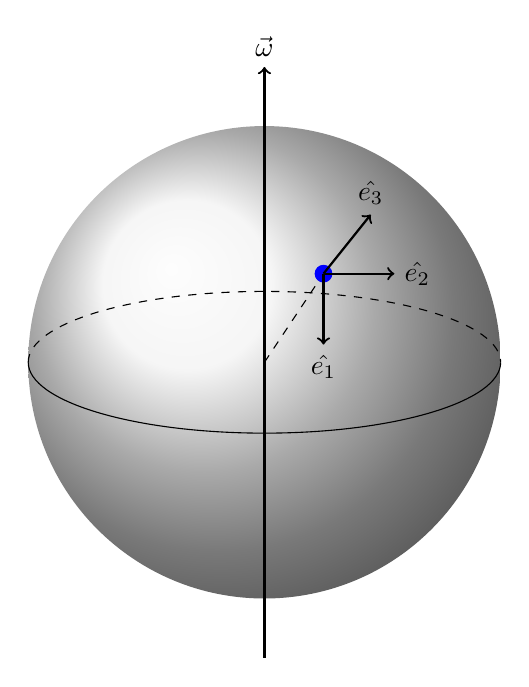
\begin{tikzpicture}[scale=1.5]
        % Draw the sphere
        \shade[ball color=gray!10] (0,0) circle (2cm);
        % Draw the axis of rotation
        \draw[thick,->] (0,-2.5) -- (0,2.5) node[above] {$\vec{\omega}$};
        % Draw the equator
        \draw (-2,0) arc (180:360:2 and 0.6);
        \draw[dashed] (-2,0) arc (180:0:2 and 0.6);
        \draw[dashed] (0,0) -- (0.5,0.75);
        % Draw the point particle
        \filldraw[blue] (0.5,0.75) circle (2pt);
        \draw[thick,->] (0.5,0.75) -- (0.9,1.25) node[above] {$\hat{e_3}$};
        \draw[thick,->] (0.5,0.75) -- (1.1,0.75) node[right] {$\hat{e_2}$};
        \draw[thick,->] (0.5,0.75) -- (0.5,0.15) node[below] {$\hat{e_1}$};
    \end{tikzpicture}
\end{wrapfigure}
In the figure, the earth's rotation about its axis with angular velocity $\vec{\omega}$ is shown. The unit vectors $\hat{e}_1$, $\hat{e}_2$, and $\hat{e}_3$ are local unit vectors on the Earth's surface, where $\hat{e}_3$ is perpendicular to the surface, while $\hat{e}_1$ and $\hat{e}_2$ lie on the surface. The component of $\vec{\omega}$ along the $\hat{e}_3$ direction is $\omega_z$. A particle of mass $m$ is projected horizontally with an initial velocity $\vec{v}=v_0\hat{e}_2$ from the point indicated in the figure. Assume the Earth is a perfect sphere with radius $R$ and neglect air resistance.

\textbf{a.} Determine the direction and magnitude of the Coriolis force. --- \textit{0.6 points}

\textbf{b.} Determine the equations of motion in $\hat{e}_1$ and $\hat{e}_2$ directions by considering only the Coriolis force and velocity $\vec{v}$, neglecting free-fall which is in $-\hat{e}_3$ direction. --- \textit{0.4 points}

(Given: Coriolis force $\vec{F}_c = -2m \vec{\Omega} \times \vec{v}$)

\section*{Solution:}


